
\section{Análisis adicional: Resistencias }
El valor de las resistencias depende de la resistividad del material ($\rho$), la longitud (L)  y el área transversal (A) según la ecuación :

$R=\rho~\frac{L}{A}$.

\subsection{Resistividad}
\subsubsection{Dependencia del material}
La medida de cuánto resiste un material el flujo de cargas se conoce como resistividad.

En la tabla de la Fig.~\ref{fig:resistividad} pueden distinguirse dos grupos según su comportamiento eléctrico. Por un lado están los metales que son buenos conductores, como la plata, el cobre, el aluminio y el oro, que tienen resistividades muy bajas. Esa característica los hace excelentes para cables y conexiones, porque dejan pasar corriente con poca pérdida. Sin embargo, debido a esa misma razón no son los mejores materiales para fabricar resistencias, ya que para obtener un valor resistivo apreciable harían falta longitudes grandes o secciones muy pequeñas. Por otro lado, aparecen materiales como la Manganina y el Nicromo, que tienen resistividades mucho mayores que las de los metales. Esa resistividad más alta permite construir resistencias de valor útil en tamaños pequeños.

\begin{figure}[H]
\centering
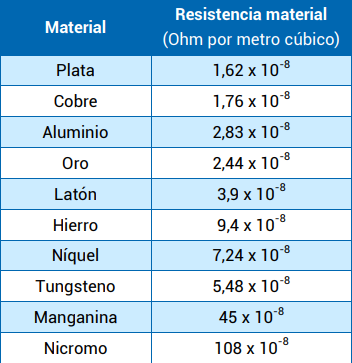
\includegraphics[width=0.6\textwidth]{resistividad.png}
\caption{Resistividad de Metales y Aleaciones a 20° C.}
\label{fig:resistividad}
\end{figure}

\subsubsection{Dependencia de la temperatura}
La resistividad de algunos materiales tiene una fuerte dependencia de la temperatura. 

En la mayoría de los metales conductores, como el cobre, la resistividad aumenta con el aumento de la temperatura. Este efecto se debe al aumento de la temperatura provoca un incremento de las vibraciones de los átomos en la estructura reticular de los metales, lo que dificulta mas el movimiento de los electrones.

En otros materiales, mayormente no conductores, la resistividad disminuye al aumentar la temperatura, convirtiéndose en mejores conductores a mayor temperatura. Esto se debe a que el aumento de la agitación térmica incrementa el número de cargas libres disponibles para transportar la corriente.


En muchos materiales, la dependencia es aproximadamente lineal y puede modelarse mediante una ecuación lineal:

$\rho= \rho_0 ~[1+\alpha(T-T_0)]$

Donde $\rho$ es la resistividad del material a la temperatura T, $\alpha$ es el coeficiente de temperatura del material y $\rho_0$ es la resistividad del material a temperatura $T_0$.

 Los metales puros suelen tener un coeficiente térmico de resistencia bastante elevado, por lo que su resistividad cambia considerablemente cuando aumenta su temperatura. En cambio, los materiales como la Manganina (aleación de Cu, Mn, Ni) y el Nicromo (aleación de Ni, Fe, Cr) presentan un coeficiente térmico de resistencia pequeño, por lo que su resistencia cambia poco aunque se calienten.
 
 \subsubsection{Conclusión}

En consecuencia, cuando se fabrican resistencias al elegir el material que se va a utilizar no solo importa que tengan una resistividad adecuada, sino también que su valor permanezca lo más estable posible frente a los cambios de temperatura. Considerar estas cualidades es de suma importancia. Por ejemplo, a lo largo del TP conviene trabajar con materiales cuyo comportamiento sea lo más constante posible, para que las diferencias observadas se deban principalmente al circuito y a los instrumentos, y no a variaciones bruscas del material.


\subsection{Tolerancia asociada}
Toda resistencia fabricada posee una tolerancia asociada, que indica el rango de variación permitido respecto de su valor nominal. Esta tolerancia se expresa como un porcentaje y se debe a limitaciones inherentes al proceso de fabricación, como impurezas en el material, variaciones en las dimensiones geométricas y condiciones de producción.

Por ejemplo, una resistencia de $100\,\Omega$ con una tolerancia del $\pm 5\%$ puede tomar valores reales comprendidos entre:

\[
95\,\Omega \leq R \leq 105\,\Omega
\]

Este rango de incertidumbre debe tenerse en cuenta al comparar valores nominales, medidos y calculados. En particular, diferencias entre estos valores no necesariamente indican errores experimentales, sino que pueden encontrarse dentro del margen de tolerancia del componente.

En resistencias comerciales, la tolerancia suele indicarse mediante un código de colores (el Oro para el $\pm 5\%$ y la plata para el $\pm 10\%$) . Los valores más comunes son $\pm 1\%$, $\pm 2\%$, $\pm 5\%$ y $\pm 10\%$. Resistencias con menor tolerancia (mayor precisión) son más costosas y se utilizan en aplicaciones donde se requiere mayor exactitud.

En el marco del trabajo práctico, la tolerancia de las resistencias contribuye a las discrepancias entre los valores nominales y los obtenidos experimentalmente.

\subsection{Resistencias comunes}
\begin{itemize}
    \item Resistencias de películas de carbono: El material resistivo se deposita sobre un soporte cerámico. Fue uno de los materiales más utilizados en resistencias debido a su bajo costo, su facilidad de fabricación y su amplio rango de valores resistivos. En la actualidad es muy útil para las resistencias de uso general que no buscan demasiada precisión. Sin embargo, muchas han sido reemplazadas por tecnologías de película metálica, que ofrecen mejor tolerancia y estabilidad pero mas costosas.

    \item Resistencias de Manganina: Se emplea principalmente en resistencias de precisión y resistencias de sensado de corriente. Esto debido a que posee un coeficiente térmico muy bajo, del orden de $±0.000015 °C $.

    \item Resistencias de Nicromo: Se usa principalmente en elementos calefactores y resistencias bobinadas. Tiene resistividad alta, buena estabilidad a temperatura elevada y gran resistencia a la oxidación, debido a que al calentarse forma una capa protectora de óxido que lo preserva del deterioro rápido con el aire.
\end{itemize}

\subsection{Fuentes}
\begin{itemize}

     \item Física universitaria volumen 2, 9.3 Resistividad y resistencia. 17 nov 2021. OpenStax. \url{https://openstax.org/books/f%C3%ADsica-universitaria-volumen-2/pages/9-3-resistividad-y-resistencia}
       \item ELECTRÓNICA Guía de estudio 1:
¡Resistiré!. Instituto Nacional de Educación Tecnológica. \url{https://www.inet.edu.ar/wp-content/uploads/2020/07/ELECTRONICA_Gu--a01-Resistencias.pdf}
    
    
\end{itemize}